\section{多主体模型与历史检验}
\subsection{主体属性、行为与信息}
系统由四类有用服务载能群、七类发电投资单元、两类储能投资单元、三个燃料供给单元与政府组成。载能群按煤、油、气和电设备划分。电力市场以工程边际排序和比例燃料配给清算，形成稀缺价格与利用率反馈。

每年先从既有建设队列投产并退役，再根据历史形成的预期提出服务请求，按实际容量与料源清算。随后投资主体根据利润、利用率创新、弃电及服务缺口下单，政府根据排放误差更新下一年碳价。模型保存217个内生状态，其中180维为12类资产的15个未来投产槽。



\begin{table}[!htbp]\centering\small\caption{主体的可观察属性与实际决策}\begin{tabularx}{\textwidth}{lXX}
\toprule
主体 & 状态/接收信息 & 改变系统的动作 \\\midrule
消费载能群 & 设备份额、预期需求、相对成本、上一年缺供 & 在流量计算前改变四种载能请求份额 \\
发电/储能投资 & 装机、在建、利润、利用率、弃电与短缺 & 提出毛订单并在共同资金和建设上限内下单 \\
燃料供给 & 生产能力、进口渠道、库存与直接/发电领用 & 实际供给、库存释放与后续能力订单 \\
政府 & 实际模型排放、参考路径、既有碳价 & 改变下一期碳价，不能直接强迫净零 \\
运行清算环境 & 可用电源与同载能资源竞争 & 实现发电、直接交付、缺供、收益和稀缺信号 \\
\bottomrule
\end{tabularx}
\end{table}

\subsection{预期与载能选择}
有用服务$U_t$与电力预期由历史低维规则形成；候选为近期增量、GDP弹性和强度漂移，按每个训练起点以前的内层滚动结果选择。预期形成服务请求，装机与供给随后按物理状态实现。设$b_{f,t}$为基准预期份额，$z_{f,t-1}$为上一期缺供比例，目标份额与调整为
\begin{align}
q_{f,t}&=\operatorname{softmax}_f\{\log b_{f,t}-\beta_c\Delta c_{f,t}-\beta_z z_{f,t-1}\},\\
\tilde s_{f,t-1}&=\operatorname{norm}_f\{b_{f,t}s_{f,t-1}/b_{f,t-1}\},\quad
s_{f,t}=(1-\lambda)\tilde s_{f,t-1}+\lambda q_{f,t}.
\end{align}
其中成本为相对预期的变化，避免把固定价差逐年重复积分；$\lambda=0.5$、响应系数属于工程行为假设。先算份额，再由$D_{f,t}=U_ts_{f,t}/(\eta_f\chi)$计算直接燃料请求，$D^E_t=U_ts_{E,t}/\eta_E$计算电力请求，$\chi=29.3076/3.6$ TWh/Mtce。主动响应关闭时设$s=b_t$，保留自主趋势；独立的冻结份额诊断在流量计算前固定$s=s_{2024}$，同时移除趋势与响应。

\subsection{建设、退役与共同资本}
发电、储能和供给能力由物理存量演化：
\begin{align}
K_{j,t}&=(1-\delta_j)K_{j,t-1}+Q^{(1)}_{j,t-1},\\
Q^{(\ell)}_{j,t}&=Q^{(\ell+1)}_{j,t-1}+I_{j,t}\mathbf1\{\ell=L_j\},\qquad Q^{(16)}=0,\\
I_{j,t}&=\bar I_{j,t}\min\{1,B_t/\sum_k c_{k,t}\bar I_{k,t}\},\quad
\sum_jc_{j,t}I_{j,t}\le B_t.
\end{align}
本年末订单$I_{j,t}$经建设后供能；例如2025年下单、五年工期在2030年投产。基准工期煤/气2年、核5年、水4年、风2年、光1年、生物质2年、电池1年、抽蓄4年，燃料供应2/3/2年。历史容量差是净增，参考毛订单须加声明退役补偿。初始队列按近期吞吐推算，为后续建设时序提供工程初态。

期望订单由近期净增锚、退役补偿以及实际运行创新构成，利润响应以起点已知的市场价格与技术利用率构造参照回报，再与当年实际回报比较，避免实际市场价格和实际发电量在差分中被共同抵消。优先权仅乘在期望订单上，之后依次接受生物质料源、年度建设上限和共同资本约束，再进入建设队列。基准资本规模采用工程代理。成本下降作用于风、光、生物质和电池的资本系数，终端装机由实际订单逐期形成。



\begin{figure}[H]\centering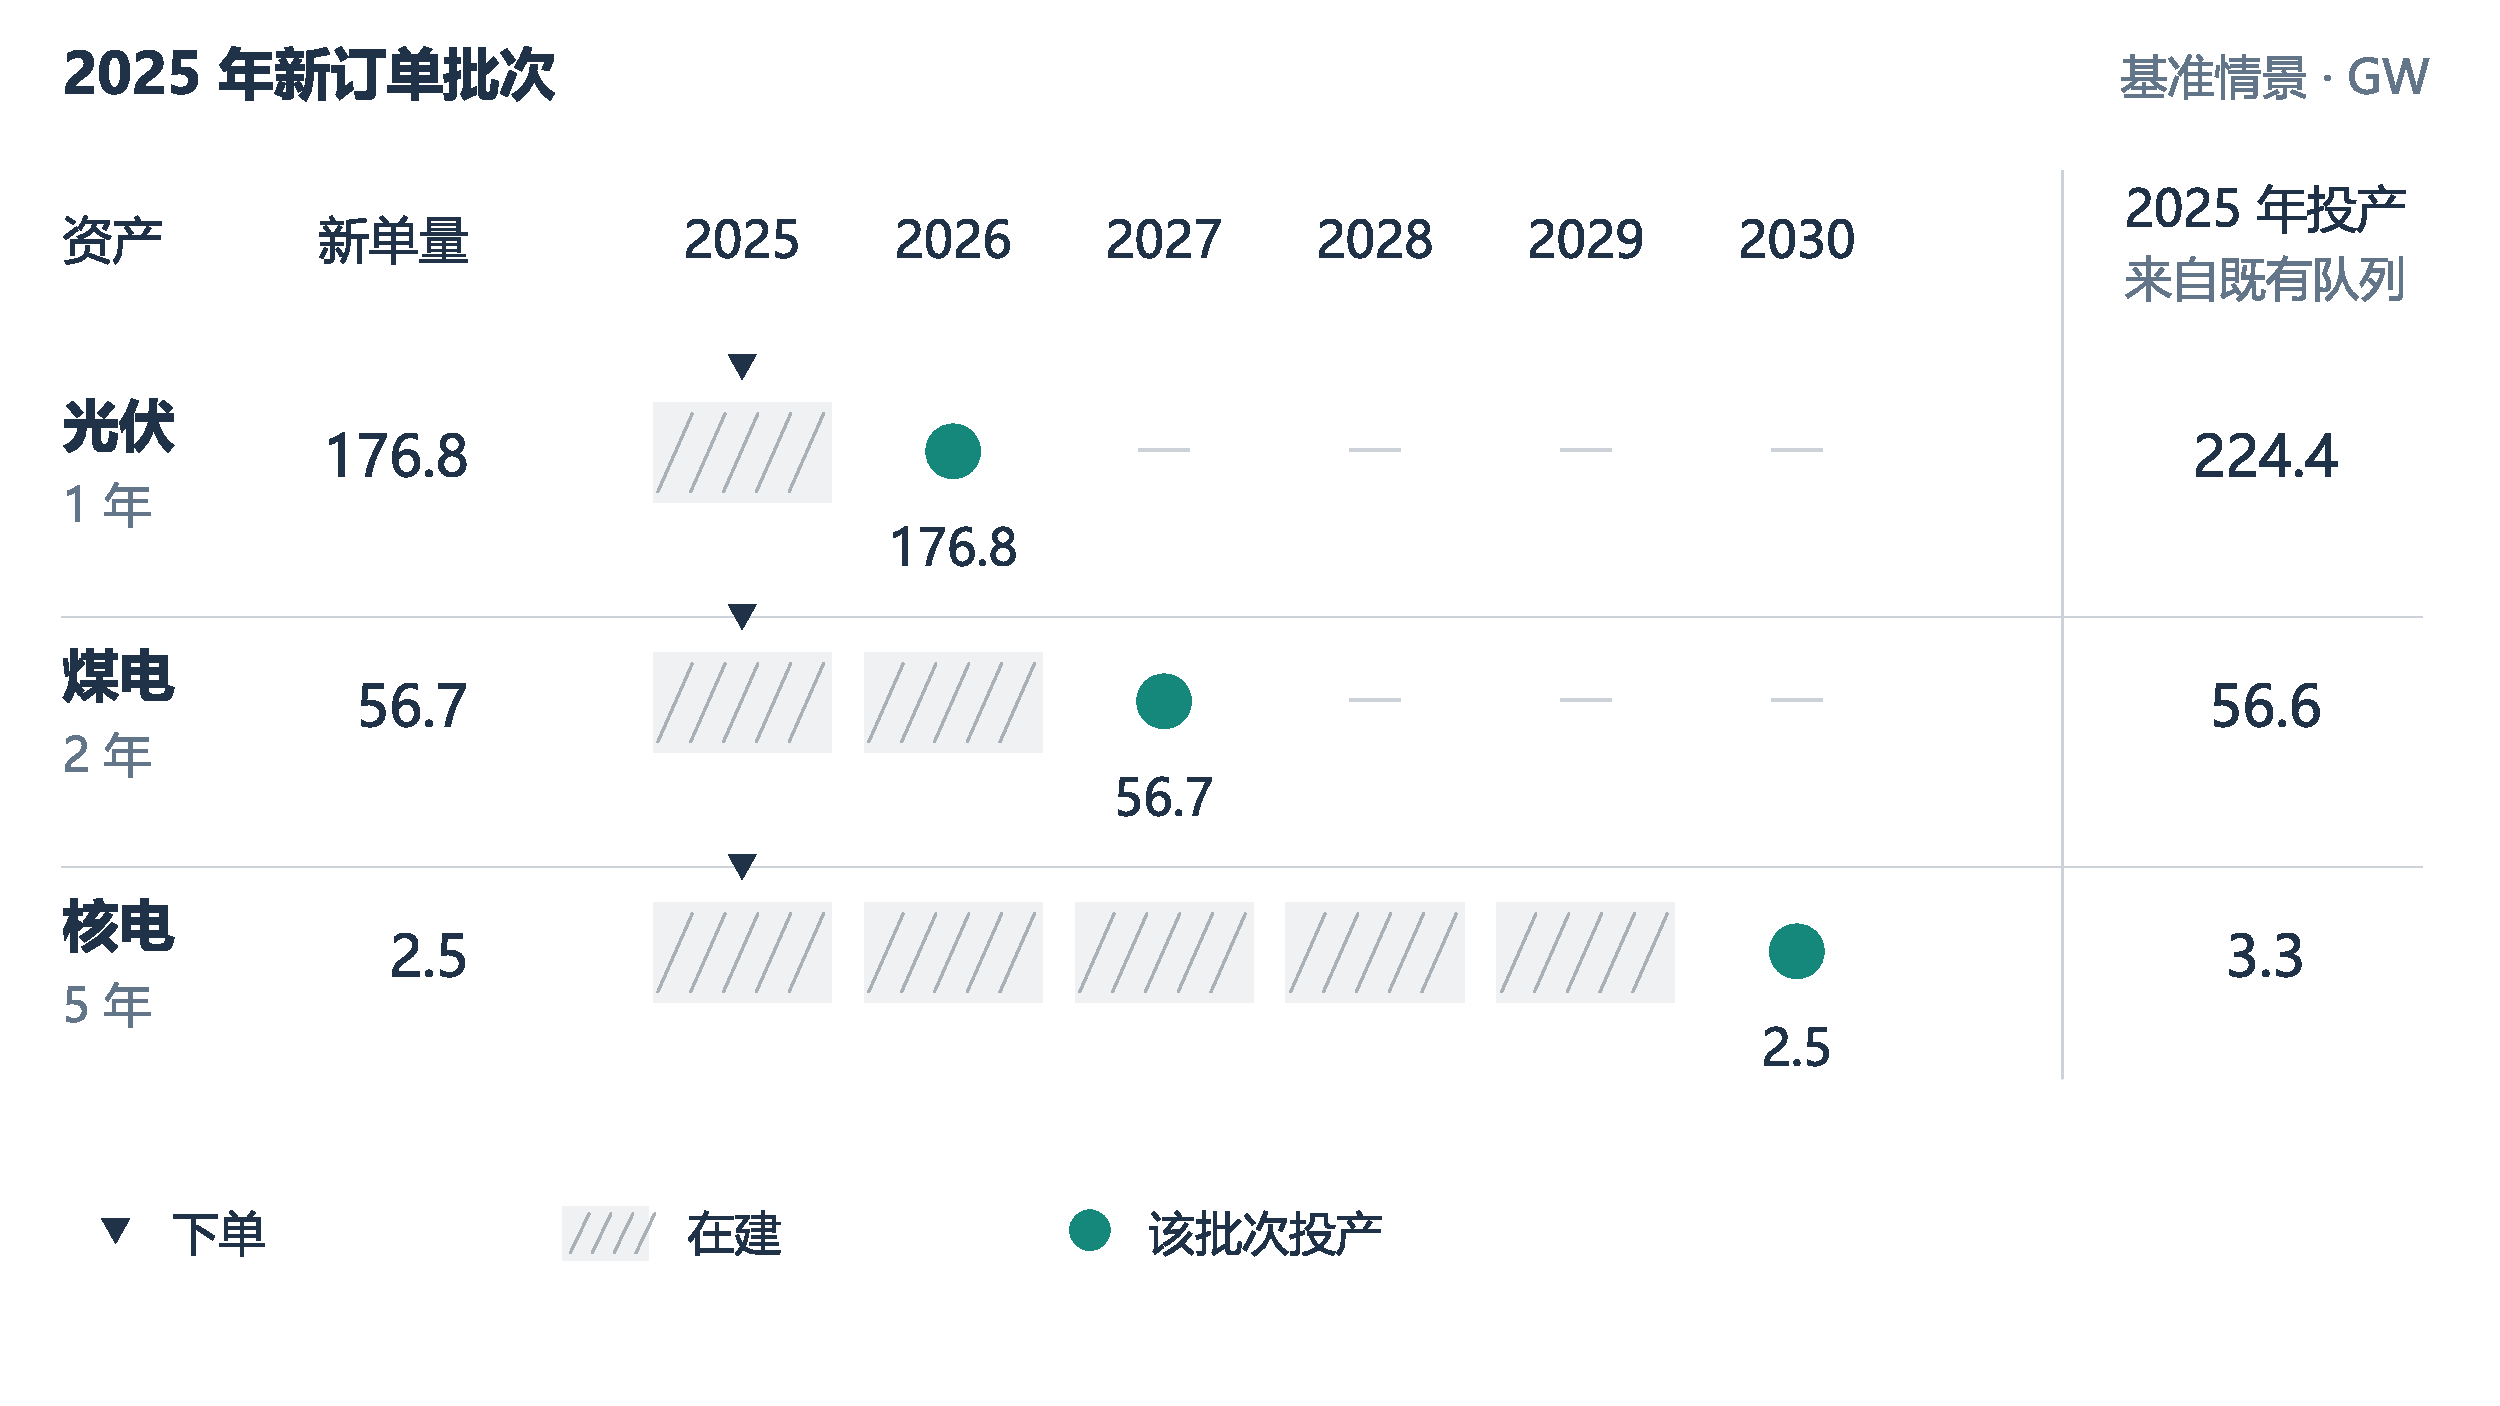
\includegraphics[width=\linewidth]{figures/fig02_queue_matrix.pdf}\caption{建设队列矩阵：2025年订单经过各技术工期后投产；同年投产的既有项目单列，避免将初始在建量归入新订单。}\label{fig:fig02_queue_matrix}\end{figure}
\subsection{可解释的投资收益响应}
投资主体的实际利润与参照利润必须由不同信息集形成。对发电技术$j$，以起点已知的利用率$u_{j,0}$、市场价$p_0$、碳价$c_0$和资本系数$C_{j,0}$构成每单位装机的参照回报，而非同时代入实际市场价与实际发电量：
\begin{align}
\pi_{j,t}&=G_{j,t}(p_t-v_j-c_t e_j)-0.08C_{j,t}K_{j,t},\\
\pi^{\rm ref}_{j,t}&=K_{j,t}\{8.76u_{j,0}(p_0-v_j-c_0e_j)-0.08C_{j,0}\},\\
\rho_{j,t}&=\frac{\pi_{j,t}-\pi^{\rm ref}_{j,t}}{\max(0.08C_{j,0}K_{j,t},1)},\qquad
m_{j,t}=\operatorname{clip}(1+0.25\rho_{j,t},0,2).
\end{align}
$G$为TWh、$p$为元/MWh，故利润以百万元计；$e_j$为年度有效燃烧映射下的排放系数。起点市场价450元/MWh、碳价100元/吨为工程初态。$m$只修正期望订单，之后仍要通过共同资本与建设上限；利用率创新、短缺及弃电另作用于订单反馈。收益响应系数0.25与8\%年资本费用为工程行为设定。该规则使当期市场价格和利用率改变后续订单，保供与排放效应由完整动态实验检验。

\subsection{独立进口渠道与基年资源闭合}
对燃料$f$，以观测国内生产$P_{f,0}$、观测消费$C_{f,0}$和独立总进口$I_{f,0}$确定国内留用比例：
\begin{equation}
r_f=(C_{f,0}-I_{f,0})/P_{f,0},\qquad 0\le r_f\le1,\qquad r_fP_{f,0}+I_{f,0}=C_{f,0}.
\end{equation}
进口渠道与国内生产能力分别演化，$r_f$作用于国内可用供应。$P_{f,0}+I_{f,0}-C_{f,0}$作为模型平衡调节项单列。进口实物量采用官方来源，折标采用工程参考：煤0.7143 tce/t，原油1.4286 tce/t，天然气1.2143 kgce/m$^3$\cite{ndrc_conversion,nbs_conversion}；成品油聚合按燃料油系数1.4286 tce/t代表。该映射同时保留煤进口和国内供应约束。

\begin{table}[H]\centering\caption{2024年三燃料的独立进口与初态闭合（Mtce）}
\begin{tabular}{lrrrr}\toprule
燃料 & 国内生产 & 总进口 & 留用比例 & 模型供应\\\midrule
煤 & 3,182.22 & 387.65 & 0.8746 & 3,170.72 \\
油 & 303.78 & 859.52 & 0.7413 & 1,084.72 \\
气 & 308.76 & 220.64 & 0.9841 & 524.48 \\
\bottomrule\end{tabular}\end{table}
\noindent{\small 表中容量、流量与留用比例按展示位数舍入，模型供应使用未舍入值计算并闭合。}\par
\subsection{燃料账与政策反馈}
煤、油、气各有独立守恒式
\begin{equation}
S_{f,t}=S_{f,t-1}+P^{\rm in}_{f,t}+M^{\rm in}_{f,t}-C^D_{f,t}-G_{f,t}/(\eta^G_f\chi).
\end{equation}
$P^{\rm in}$与$M^{\rm in}$为实际进入资源账的国内和进口流量，分别受可用上界限制；国内上界为$r_fP_{f,t}\mu^P_t$。同一燃料的直接使用与发电领用竞争当期可用供给，短缺时按请求比例配给。正常进口渠道$K^M_{f,t}$随经济规模演化，当年有效可用上界为$M^{\rm avail}_{f,t}=K^M_{f,t}\mu^M_t\eta^{\rm shock}_{f,t}$；进口倍率$\mu^M$与冲击保留率$\eta^{\rm shock}$作用于当年流量。库存补充不超过供给余量与声明补充速率。生物质发电既受容量限制，也受独立可发电料源预算限制，且该预算传入小时层。

年度排放为按历史宏观燃料消耗识别的有效映射，另加简化工业过程项。政府更新
\begin{equation}
p^C_{t+1}=\operatorname{clip}\{p^C_t+d_C+\kappa(E^N_t/E^R_t-1),\,0,\,2000\}.
\end{equation}
参考路径$E^R_t$仅影响控制误差，不直接规定真实排放。固定碳汇为800 Mt/年；模型净CO$_2$为能源与简化工业合计减该碳汇，未安装CCS。剩余移除需求$\max(E^N_t-800,0)$量化现有技术组合与目标之间的缺口。


\subsection{共享预期模块的历史检验}
以一年距2017—2023年七个起点、三年距2017—2021年五个起点检验服务预期与资产演化组件。各起点只用已有历史校准，并条件给定之后已实现GDP；动态主体、近期三年净增和持平采用同一目标。该组件沿用共享的既有预期与资产逻辑，2024年独立进口映射仅用于当前初态的前瞻试验。

\begin{figure}[H]\centering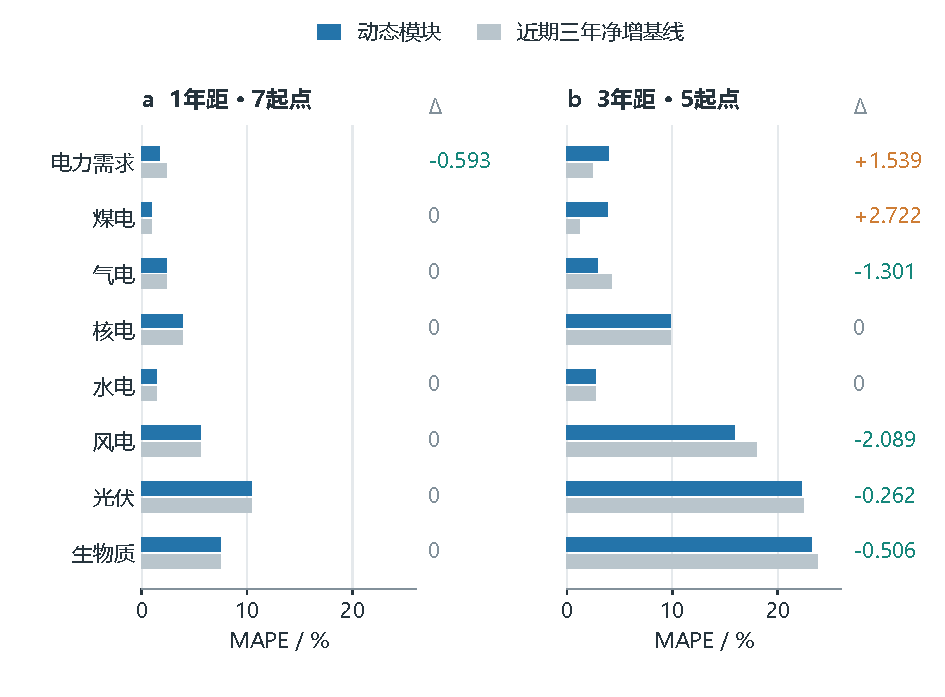
\includegraphics[width=\linewidth]{figures/fig03_validation.pdf}\caption{历史滚动验证的绝对误差与相对改进。两列同尺度横条分别为动态模块和近期三年净增基线的MAPE，右列$\Delta$为动态减基线，单位百分点；负值表示动态误差较低。全部8目标、16项比较保留；一年距7个、三年距5个起点。一年距7项容量及三年距核电、水电的两臂逐起点预测在数值精度内相等，|$\Delta$|$\le$$10^{-12}$显示0，图中其余差值保留3位小数。验证针对共享预期/资产组件，条件给定已实现GDP。}\label{fig:fig03_validation}\end{figure}

\begin{table}[H]\centering\caption{共享预期模块电力需求MAPE（\%）}
\begin{tabular}{lrrr}\toprule
预测年距 & 动态主体组件 & 近期净增 & 持平\\\midrule
1 & 1.713 & 2.306 & 5.855 \\
3 & 3.992 & 2.452 & 15.916 \\
\bottomrule\end{tabular}\end{table}

一年电力误差低于近期净增，三年则高于该基线；风光及生物质快速增长时的中期偏差更大。组件验证帮助确定条件推演的适用范围，完整资源模型另通过基年资源闭合、状态守恒和机制对照检验。
\FloatBarrier
